\section{Problem 1}

\subsection{Problem 1 (a)}
    \label{sec:a}
    The matrix form of this Hamiltonian can be obtained by comparing explicitly in calculation
    
    \begin{align}
        &\begin{pmatrix}[1.5]
            b^\dagger_0 & b^\dagger_1 & \hdots & b^\dagger_{L-1} & b^\dagger_\odot
        \end{pmatrix}
        \begin{pmatrix}[1.5]
            M_{0,0} & M_{0,1} & \hdots & M_{0,L-1} & M_{0,L} \\
            M_{1,0} & M_{1,1} & \hdots & M_{1,L-1} & M_{1,L} \\
            \vdots & \vdots & \ddots & \vdots & \vdots \\
            M_{L-1,0} & M_{L-1,1} & \hdots & M_{L-1,L-1} & M_{L-1,L} \\
            M_{L,0} & M_{L,1} & \hdots & M_{L,L-1} & M_{L,L}
        \end{pmatrix}
        \begin{pmatrix}[1.5]
            b^\dagger_0 \\ b^\dagger_1 \\ \vdots \\ b^\dagger_{L-1} \\ b^\dagger_{\odot}
        \end{pmatrix} \\
        & = \underbrace{\sum_{i=0}^{L-1} b^\dagger_i M_{ii} b_i}_\text{diagonal} + \underbrace{\sum_{i\neq j}^{L-2} b^\dagger_iM_{ij}b_j}_\text{rest} + \underbrace{\sum_{i=0}^{L-2} b^\dagger_iM_{iL}b_\odot}_\text{rightmost col \textbackslash diag} + \underbrace{\sum_{i=0}^{L-2} b^\dagger_\odot M_{Li}b_i}_\text{bot row \textbackslash diag}
    \end{align}
    
    Since the operators on different sites commute, the matrix entries can be read off the Hamiltonian as 
    \begin{align}
        \begin{pmatrix}[1.3]
            0 & -t & \hdots & -t & -s \\
            -t & 0 & \hdots & -t & -s \\
            \vdots & \vdots & \ddots & \vdots & \vdots \\
            -t & -t & \hdots & 0 & -s \\
            -s & -s & \hdots & -s & 0
        \end{pmatrix}
    \end{align}
    This $(L+1) \times (L+1)$ matrix is diagonalised for a sample of values of $\nicefrac{s}{t}$. As previously mentioned in the implementation section, this is done by setting $t=1$ and varying $s$, which can be interpreted as expressing the center hopping strength s in units of on-wheel hopping strength $t$. We obtain a set of eigenvalues for each hopping strength $s$. The eigenvalues are sorted by magnitude and plotted. The largest and smallest eigenvalue are always coloured individually, all others have the same colour. \autoref{fig:spectrum_manual} shows the log-linear plot for $L = 2$ up to $11$, corresponding to $12$ sites in total with the center.

    The first observation is the fact that all plots are similar. While the number of eigenvalues increases, there are only three distinct "trajectories": the first and last eigenvalue split up, while all other eigenvalues are constant on a line. When the last eigenvalue and the constant eigenvalues cross, the colours swap since the eigenvalues are ordered by magnitude. 
    
    Theoretically, it could be possible to keep track of the eigenvalues correctly by calculating the derivatives at the crossing to identify each eigenvalue. However, it was not immediately clear to us how to do that and so we decided against doing it due to time constraints. 
    
    The most important feature is that the splitting increases in magnitude as the number of sites go up. One minor observation is the fact that the first and last eigenvalues start out symmetrically spaced around 0 for $L=2$, but the ground state drops with increasing $L$ right from the smallest $\nicefrac{s}{t}$ value. 
    
    In short, as $L$ increases, the split off of the ground state increases and the initial ground state energy decreases.

    \begin{figure}[!t]
        \centering
        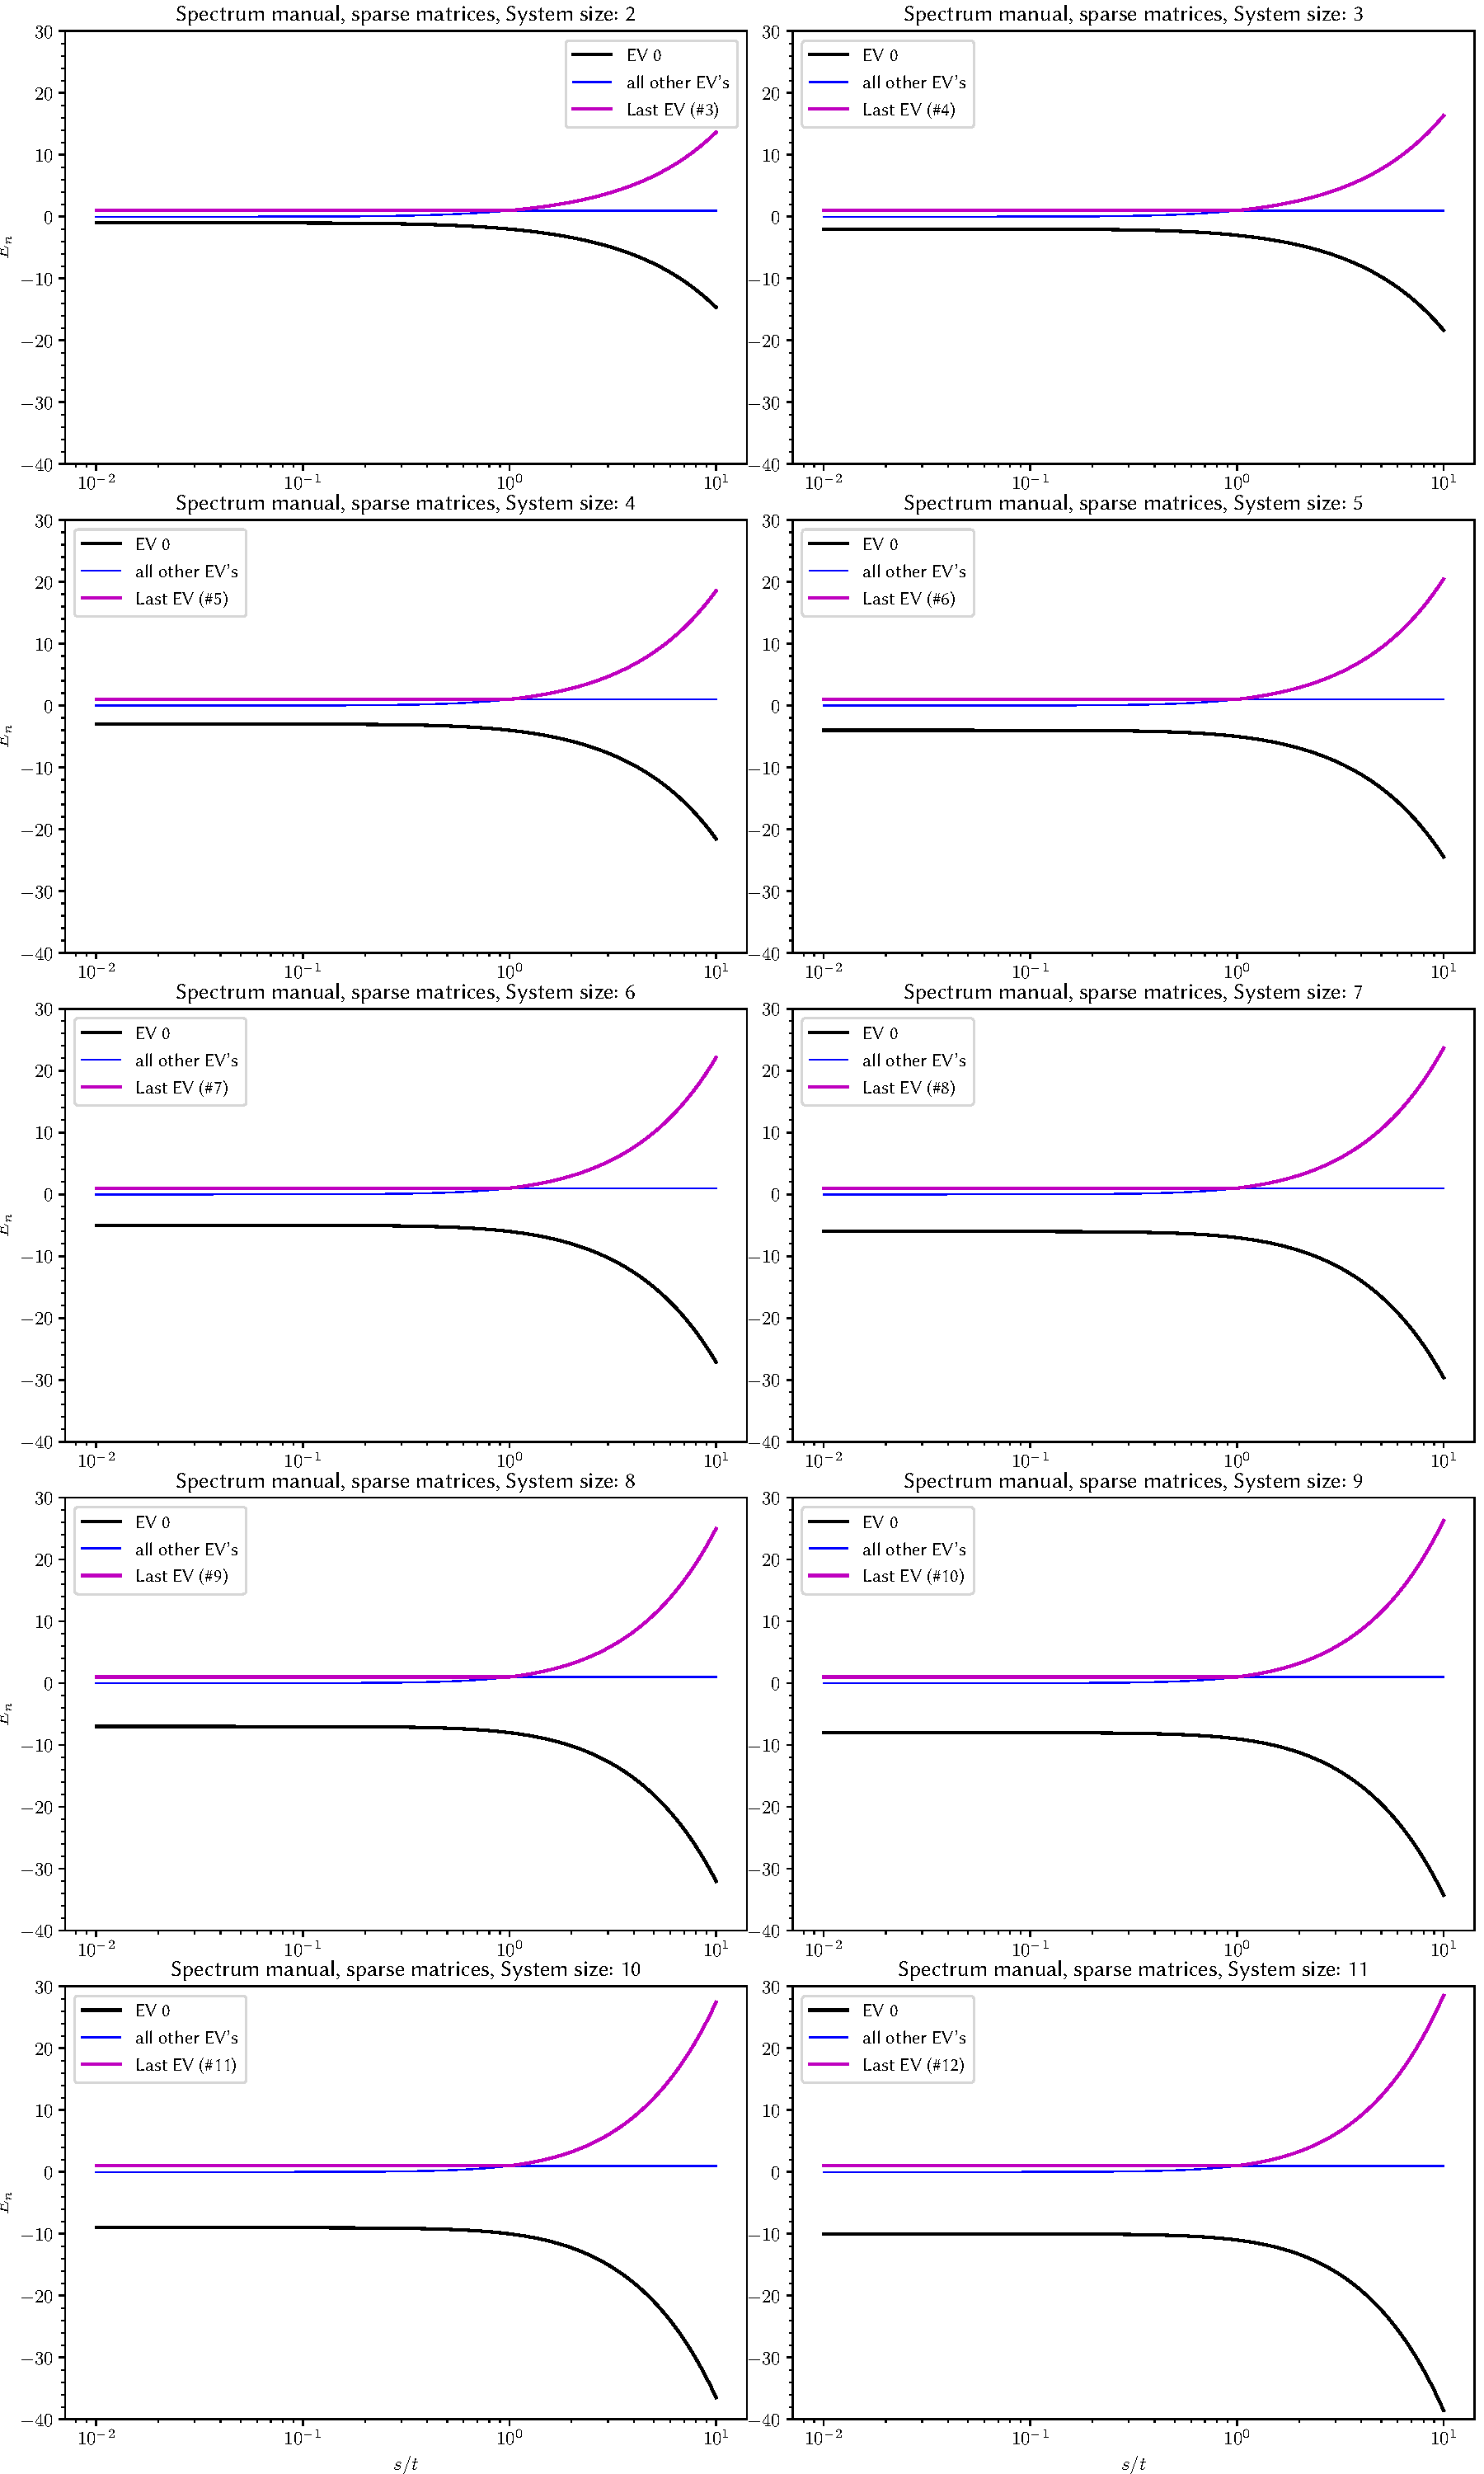
\includegraphics[width=\textwidth]{graphics/spectrum_manual.pdf}
        \caption{Spectrum of singe-particle Hamiltonian for different system sizes}
        \label{fig:spectrum_manual}
    \end{figure}
    \clearpage

\subsection{Problem 1 (b)}
    \label{sec:b}
    It is simple to check that the following identifications from  \cite{Streib} satisfies the commutation relations proposed in the problem statement:
    \begin{align}
        \hat{h_i} = \hat{S}^+_i \hspace{20pt} \hat{h_i}^\dagger = \hat{S}^-_i \hspace{20pt} \hat{S}^\pm_i = \hat{\sigma}^x_i\pm\hat{\sigma}^y_i \hspace{20pt} i \in \{1, ..., L\}
    \end{align}
    We map an "empty site" to $[1, 0] =: \ket{\uparrow}$ and an "occupied site" to $[0, 1] =: \ket{\downarrow}$. The hardcore bosonic ladder operators can then be represented in the Fock basis, e.g. for four sites, $\ket{0011} \hat{=} \ket{\uparrow} \otimes \ket{\uparrow} \otimes \ket{\downarrow} \otimes \ket{\downarrow}$. This fixes the representation of the hardcore bosonic ladder operators in the Fock basis to 
    \begin{align}
        \hat{h_i} = \hat{S}^+_i = \underbrace{\unity \otimes \unity \otimes \dotsm}_\text{i times} \otimes~\hat{S}^+ \otimes \underbrace{\dotsm \otimes \unity \otimes \unity}_\text{L-i times}
    \end{align}
    With this mapping, the Hamiltonian comes out to be a $2^{L+1} \times 2^{L+1}$ matrix. The correlator matrix takes the same size and can easily be assembled from the hardcore bosonic operators.

\subsection{Problem 1 (c)}
    \label{sec:c}
    This matrix is diagonalised for $\nicefrac{s}{t}$ values just like for Problem 1(a) (\autoref{sec:a}). The plot with the eigenvalues for up to $L=11$ is depicted in  \autoref{fig:spectrum_exact}. The first two plots are also shown magnified in \autoref{fig:spectrum_exact_subset}.
    
    The first and last eigenvalues are initially colored differently again, but they are quickly overtaken by the huge bundle of intermediate eigenvalues, which splits up into 3 major branches. Just like before, the color mapping fails at the crossings, resulting in a kink, because it was too difficult to keep track of the numerous eigenvalues (! $4095$ at $L=11$) and their derivatives on the plot. The plot essentially shows the same characteristic as the one in \autoref{fig:spectrum_manual}, with the main difference being the number of Eigenvalues and the spread. The eigenvalues start out constant as well, but additional intermediate eigenvalues start out anywhere between the first and last. Additionally, some of the intermediate eigenvalues also split up and down, essentially forming 3 bundles of eigenvalues. The spread of the bundles increases with the number of sites, and the ground state energy drops for all values of $\nicefrac{s}{t}$. For $L=11$, the plot becomes so crowded that even at negligible plotting linewidth, the bundles merge into one.
    
    \begin{figure}[b!]
        \centering
        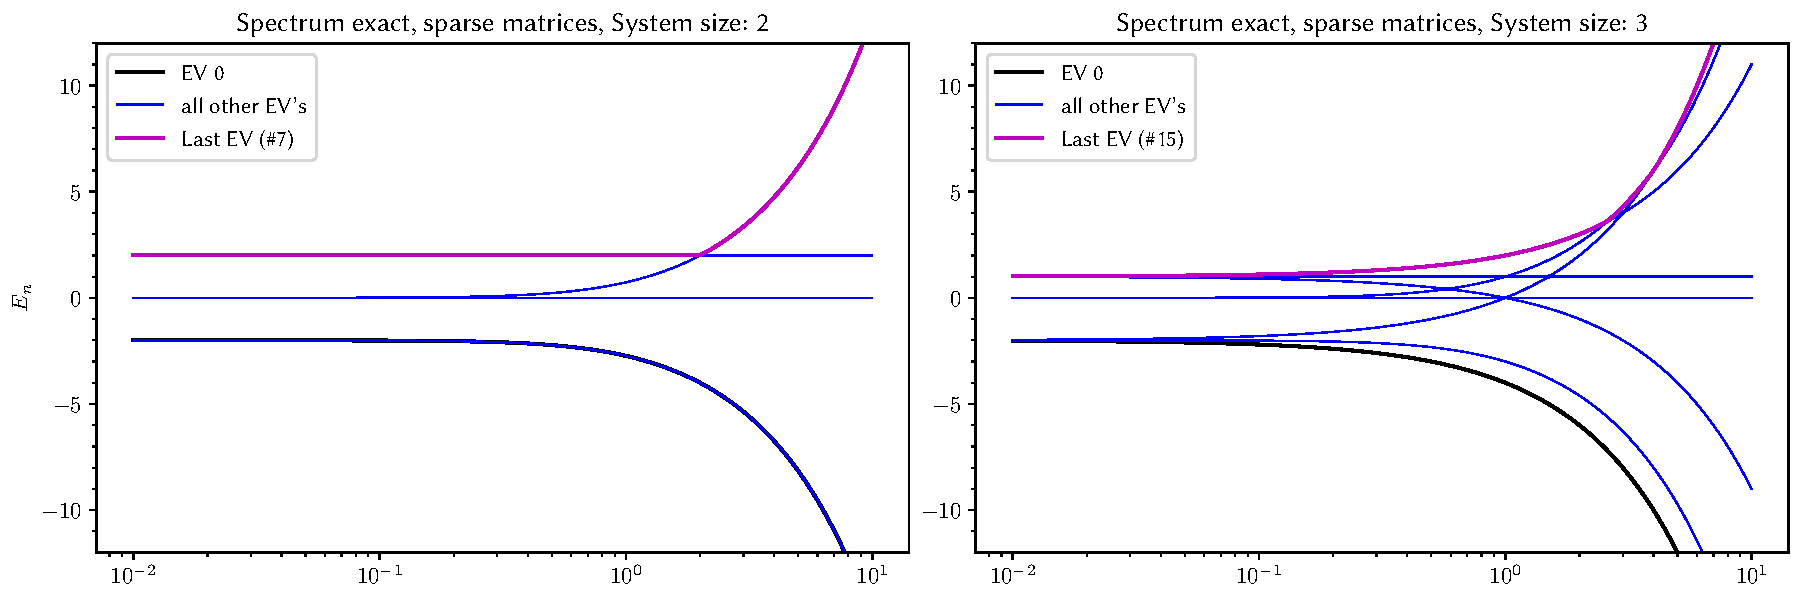
\includegraphics[width=\textwidth]{graphics/spectrum_exact_manual_subset.pdf}
        \caption{Spectrum of Hamiltonian for $L = 2, 3$, which are the first two subplots of \autoref{fig:spectrum_exact}.}
        \label{fig:spectrum_exact_subset}
    \end{figure}

    \begin{figure}[t!]
        \centering
        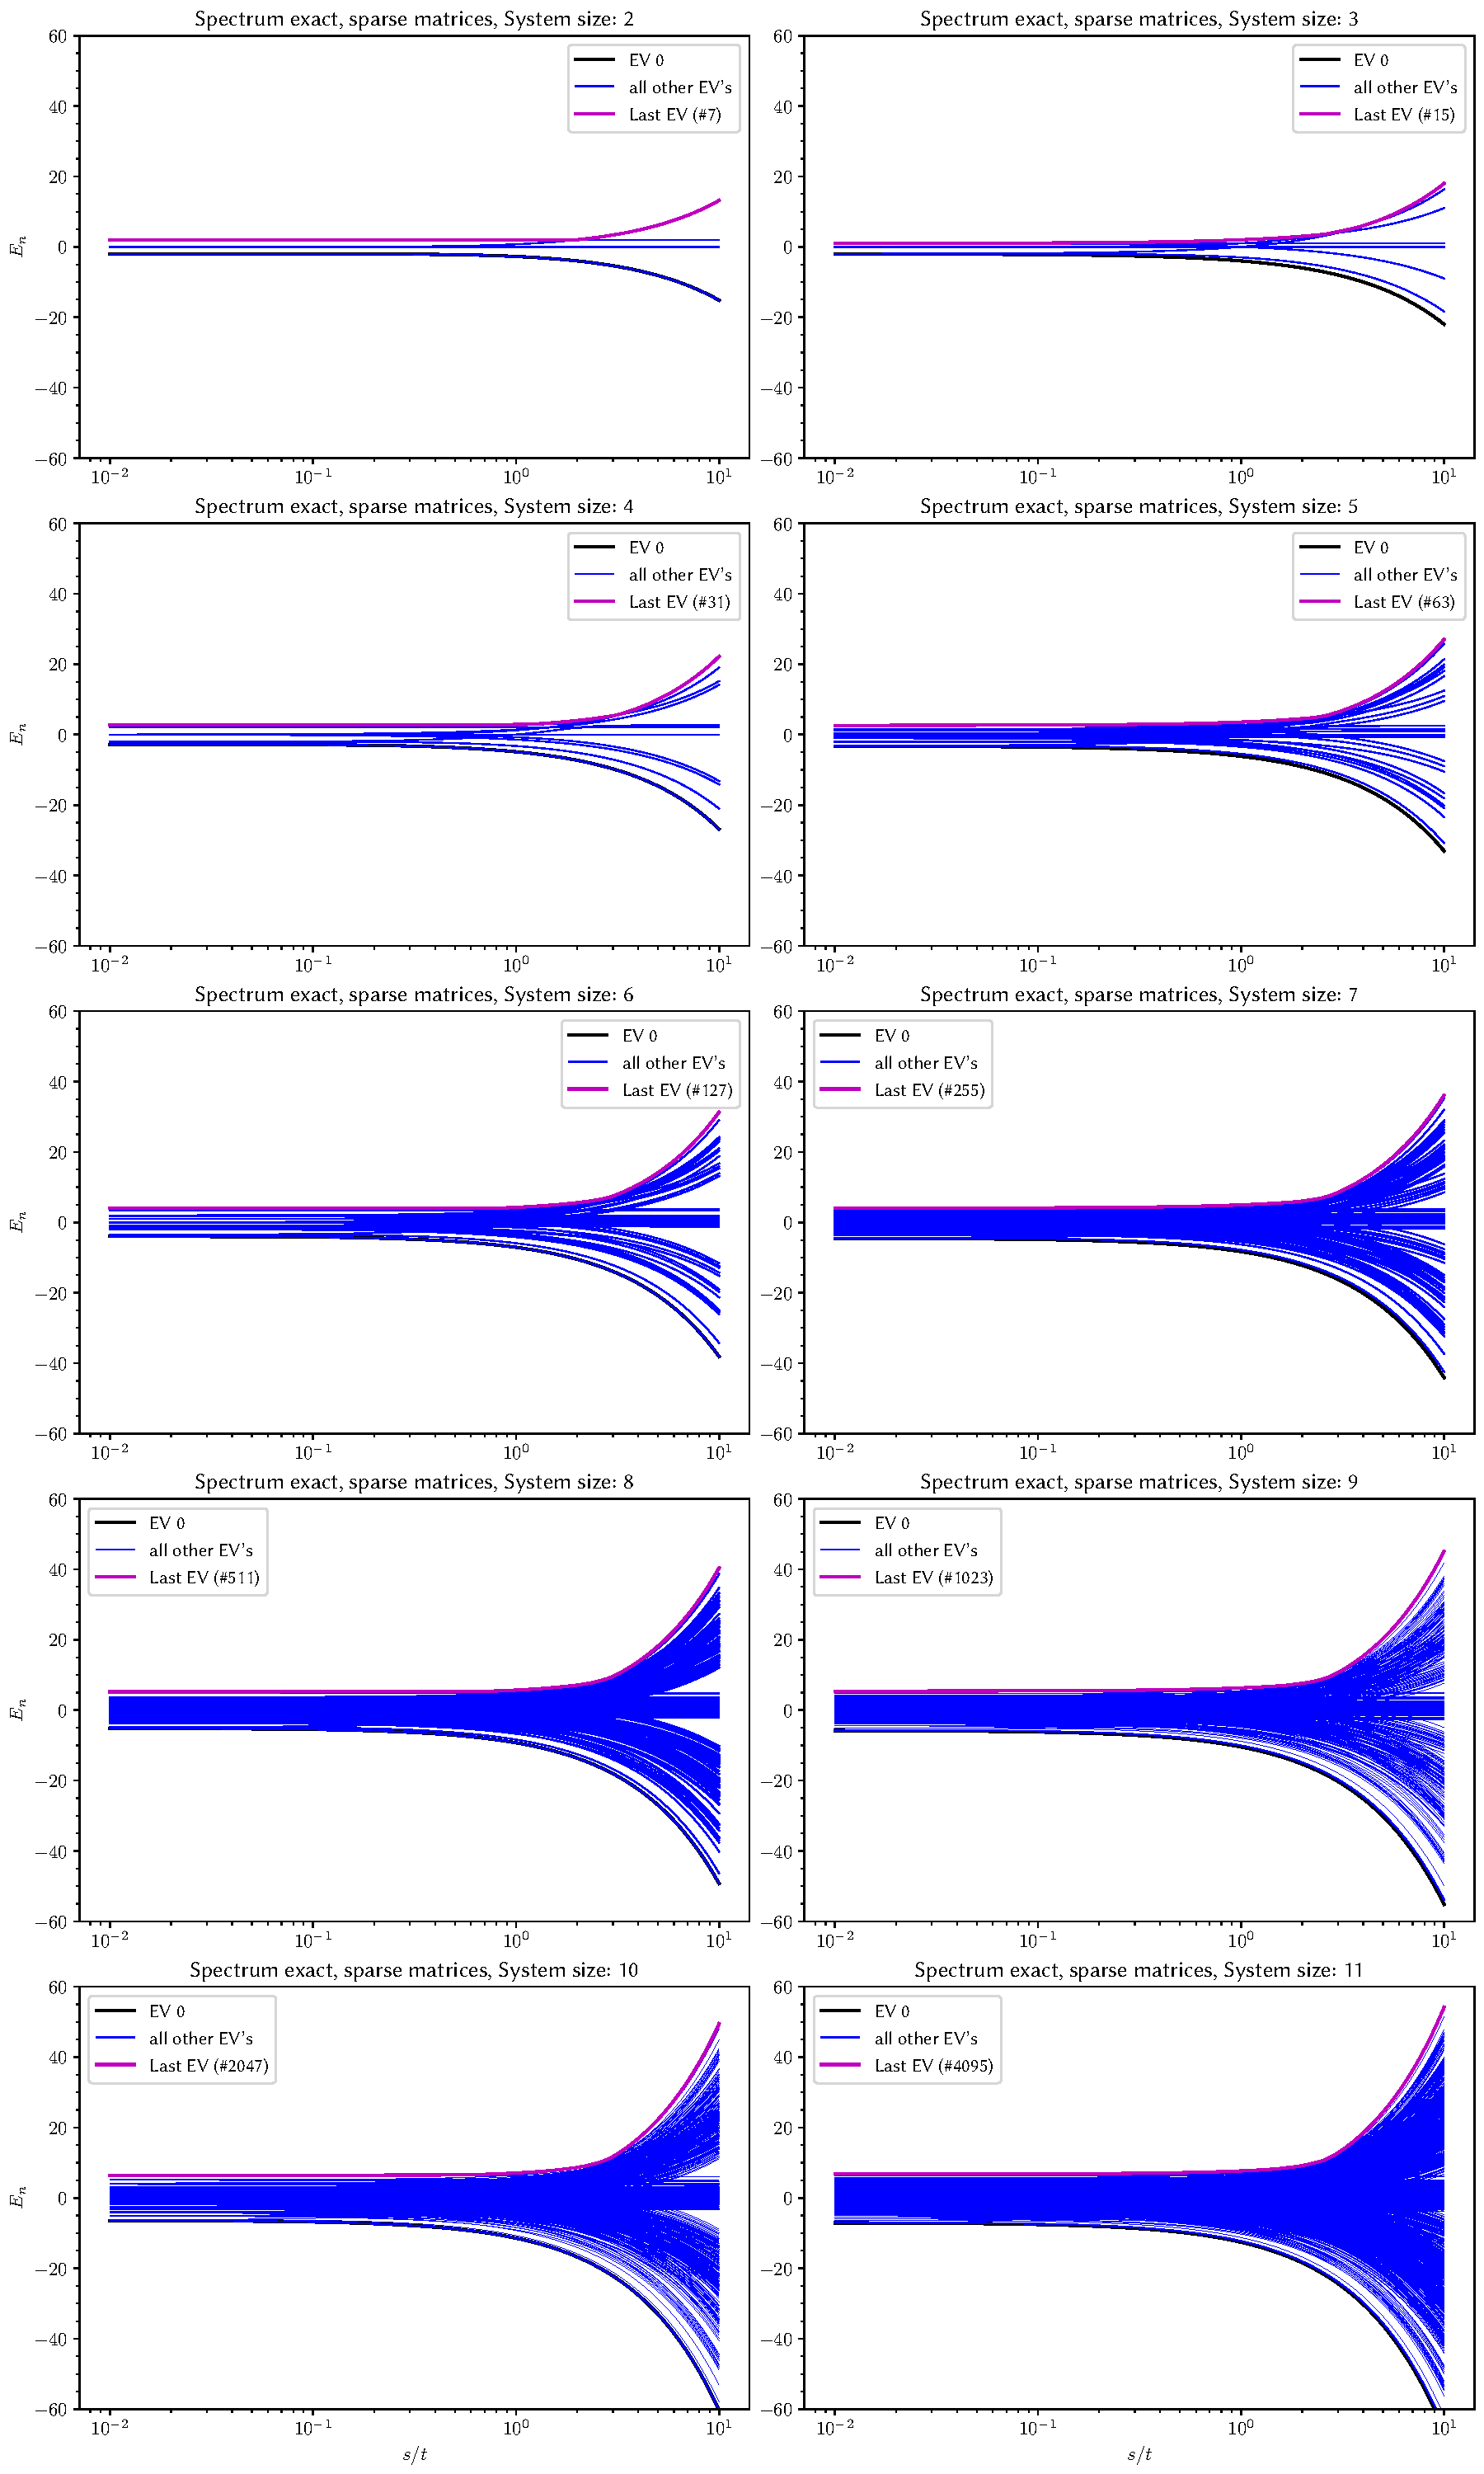
\includegraphics[width=\textwidth]{graphics/spectrum_exact.pdf}
        \caption{Spectrum of Hamiltonian for different system sizes}
        \label{fig:spectrum_exact}
    \end{figure}
    \clearpage

\subsection{Problem 1 (d)}
    \label{sec:d}
    
    To plot the condensate fraction, the Hamiltonian from Problem \ref{sec:b} and \ref{sec:c} is diagonalised again. Its ground state is easily picked as the eigenvector corresponding to the (algebraically) smallest (possibly negative) eigenvalue. The expectation value of the correlator matrix $C(i,j)$ from Problem \ref{sec:b} is then used to calculate the matrix elements of the reduced density matrix for the given $\nicefrac{s}{t}$ sample. 
    
    From the reduced density matrix, the largest eigenvalue $n_0$ corresponds to the largest number of particles that are correlated in the ground state.
    
    The trace $N$ is equivalent to the number of particles in the ground state, since the diagonal entries of the correlator are just the number operators of a site in the Fock space.
    \begin{align}
        N = \sum_j \bra{\psi_0}\hat{n}_j\ket{\psi_0}
    \end{align}
    $\rho := \frac{N}{L+1}$ is stored alongside the condensate fraction to store the filling level of the wheel. The condensation fraction is now plotted against $\frac{s}{t}$ in \autoref{fig:cond_frac}. The even and odd values of $L$ are separated to not crowd the plot. Additionally, the coloring is picked according to $\rho$, not $L$, since there are sometimes multiple trajectories visible for the same $L$.

    We observe that the condensation fractions increase in a sigmoid-like way with increasing $s/t$. In general, an increase in the condensation fraction for $\frac{s}{t} > 1$ makes sense. In this regime, the hardcore bosons prefer to hop to the center site, which is why they become increasingly correlated, since every site of the wheel is a neighbour to the center. This corresponds nicely with the regime in which the eigenvalues split in Problems \ref{fig:spectrum_manual} and \ref{fig:spectrum_exact}. As the ground state energy gets more negative (the ground state "gets cheaper"), the system's condensation rises. Globally, the even $L$ trajectories are at higher condensation fractions than the odd ones. The $L=2$ trajectory even stays constant at $1$, corresponding to a fully correlated system. Since $\rho = \nicefrac{1}{3}$ in this case, $N$ must equal $1$. Therefore there is only one particle occupying the ground state, which trivially correlates with itself, leading to a trivial condensation fraction.
            
    \begin{figure}[t!]
        \centering
        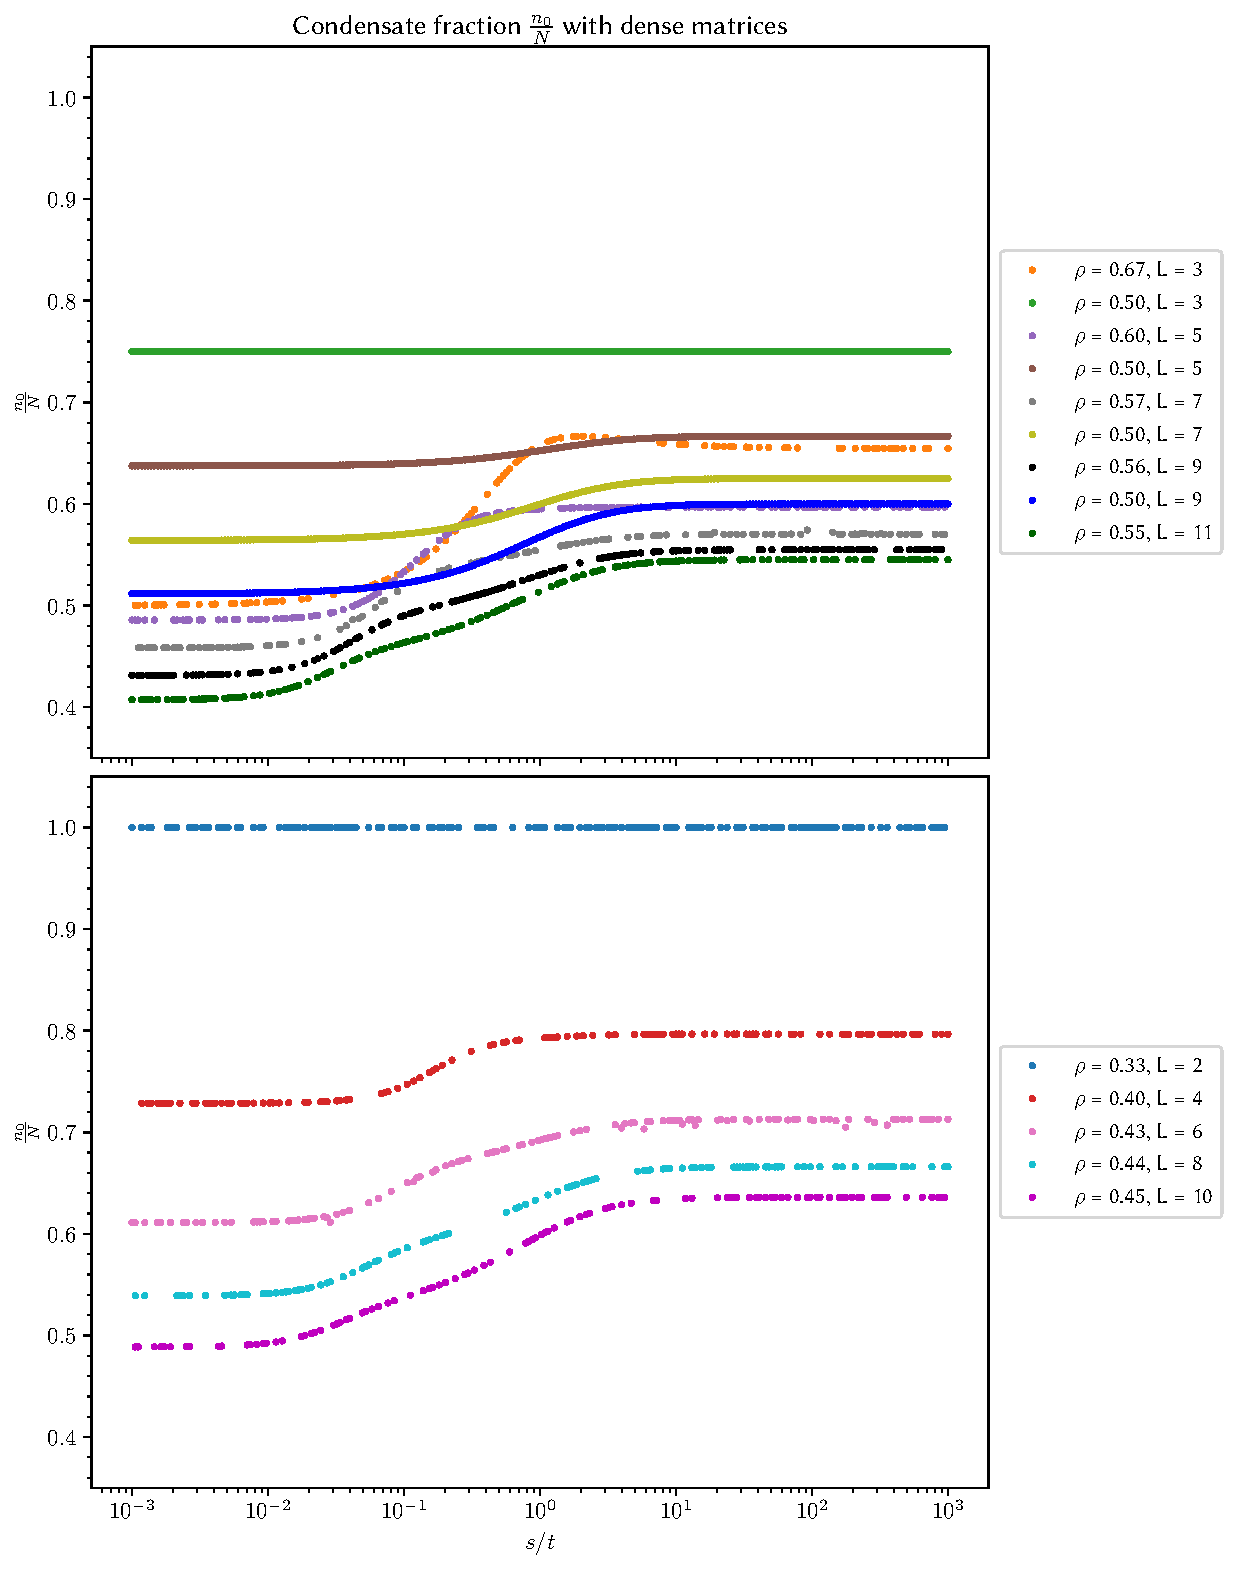
\includegraphics[width=\textwidth]{graphics/condensate_fraction.pdf}
        \caption{Condensate fractions for different number of sites and filling levels}
        \label{fig:cond_frac}
    \end{figure}
    
    We observed that all trajectories increase with growing $\nicefrac{s}{t}$ (except for tiny overshoots when settling into constant values and globally constant values). This effect is nicely illustrated on the last page in the supplementary material of \cite{wilkeSymmetryprotectedBoseEinsteinCondensation2022} in Figure S3. There, the fact that growing $s$ corresponds to higher condensate fractions is nicely illustrated across a wide range of system sizes.

    Note that the seemingly uninterrupted lines for $\rho = \nicefrac{1}{2}$ are just an artefact of the scatter plot marker size in combination with the given resolution in $\nicefrac{s}{t}$ and don't carry any physical significance.

    